\documentclass[aspectratio=169,10pt]{beamer}
\usetheme{Madrid}
\usecolortheme{default}
\usepackage{amsmath,amssymb}
\usepackage{tikz}
\usetikzlibrary{positioning,arrows.meta,shapes.geometric}
\usepackage{booktabs}
\usepackage{xcolor}
\usepackage{tabularx}

\definecolor{uavblue}{RGB}{37,99,235}
\definecolor{uavgreen}{RGB}{22,163,74}
\definecolor{uavred}{RGB}{220,38,38}
\definecolor{uavorange}{RGB}{234,88,12}
\definecolor{uavgray}{RGB}{71,85,105}
\definecolor{uavlight}{RGB}{241,245,249}

\title{Energy-Flow Feasibility and Learned Redundancy Management for Persistent K-Coverage UAV Networks}
\subtitle{Professor progress meeting --- 4 November 2026}
\author{Himanshu Nagwanshi, Surya Prakash S, Harsh Varshney, Gaddam Viswavijith}
\date{}

\begin{document}

\begin{frame}
  \titlepage
\end{frame}

\begin{frame}{Agenda (15--20 minutes)}
  \begin{enumerate}
    \item The problem, underspecification, and what the project actually is
    \item What changed: old midsem report $\rightarrow$ current report
    \item The current report: the artifact and the evaluation protocol
    \item The measured results: where learning wins, where it loses
    \item The feasibility certificate and energy ceiling
    \item Planning, distillation, classical baseline
    \item The audit and the OMNeT/INET co-simulation
    \item What is real, what is not real, and what remains open
  \end{enumerate}
\end{frame}

\begin{frame}{Executive summary}
  \begin{columns}
    \begin{column}{0.5\textwidth}
      \textbf{What this project is}
      \begin{itemize}\small
        \item A \textit{feasibility-certified evaluation study} of persistent $K$-coverage UAV-IoT over IoT sensors, with decentralized MARL control.
        \item It does \textit{not} claim RL is universally superior. It measures when learning wins, when it loses, and when the instance is infeasible.
        \item The artifact is a 25-page report plus an executable INET co-simulation and claim audit.
      \end{itemize}
    \end{column}
    \begin{column}{0.5\textwidth}
      \textbf{Where it stands}
      \begin{itemize}\small
        \item MAPPO beats the strongest rule by +0.028 on nominal (0.9512 vs 0.923).
        \item Learning wins on low connectivity (+0.125) and both failure regimes; loses on small battery and spread start.
        \item Config is \textit{not} persistently energy-feasible (ceiling 0.113 at steady state; 400 s is a finite sprint).
      \end{itemize}
    \end{column}
  \end{columns}
\end{frame}

\begin{frame}{The actual problem}
  \begin{columns}
    \begin{column}{0.48\textwidth}
      \textbf{Scenario}
      \begin{itemize}\small
        \item $N=8$ active UAVs + 1 reserve
        \item $M=20$ Gaussian sensors in an $80\times80$ m field
        \item $K=2$ required coverage; connectivity must stay intact
        \item 2 charging pads; clustered corner start; 400 s missions
        \item Actions: hover / 4 moves / charge
        \item Observation: local + communication neighbourhood + $4\times4$ deficit map + ego bearings
      \end{itemize}
    \end{column}
    \begin{column}{0.48\textwidth}
      \textbf{Why it is hard}
      \begin{itemize}\small
        \item Persistent, eventually infeasible: battery and pads cannot keep 8 UAVs up indefinitely
        \item Coverage and connectivity conflict; the swarm must stay connected while deploying across the field from one corner
        \item The deployed controller has no global state; it sees local observations only
      \end{itemize}
      \vspace{0.2cm}
      \textbf{What you are shown today}
      \begin{itemize}\small
        \item A 27-page current report with an achievability certificate
        \item An OMNeT++/INET 4.6 co-simulation at 802.11 PHY/MAC level
        \item An audit of every claim in the report
      \end{itemize}
    \end{column}
  \end{columns}
\end{frame}

\begin{frame}{The configuration we test}
  \small
  \begin{tabular}{ll}
    \toprule
    Parameter & Value \\
    \midrule
    UAVs (active + reserve) & 8 + 1 \\
    Sensors $M$ & 20 \\
    Coverage target $K$ & 2 \\
    Region $\Omega$ & $80 \times 80$ m \\
    Coverage radius $R_{\mathrm{cov}}$ & 35 m \\
    Communication radius $R_{\mathrm{comm}}$ & 40 m \\
    Altitude $z_0$ & 50 m \\
    Step $\Delta t$ & 0.2 s, $v_{\max}=5$ m/s \\
    Safety distance & 5 m \\
    Battery $B^{\max}$ & 30,000 J \\
    Hover / move / avionics & 50 W / 75 W / 5 W \\
    Charge rate & 0.0002 of pack per step \\
    Episode & 400 s (2000 steps) \\
    Deployment & connected cluster in a corner \\
    \bottomrule
  \end{tabular}
  \vspace{0.2cm}
  \begin{center}\footnotesize
    Initial deployment covers only 3 of 20 sensors; a centred ring would cover 17 and make the comparison degenerate ($CK=0.850$).
  \end{center}
\end{frame}

\begin{frame}{The two Halves of the System}
  \centering
  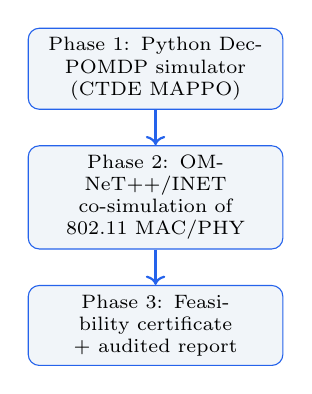
\begin{tikzpicture}[node distance=0.45cm, every node/.style={rounded corners, draw=uavblue, fill=uavlight, text width=3.0cm, align=center, font=\scriptsize, minimum height=0.62cm}]
    \node (env) {Phase 1: Python Dec-POMDP simulator (CTDE MAPPO)};
    \node[below=of env] (inet) {Phase 2: OMNeT++/INET co-simulation of 802.11 MAC/PHY};
    \node[below=of inet] (report) {Phase 3: Feasibility certificate + audited report};
    \draw[->, thick, uavblue] (env) -- (inet);
    \draw[->, thick, uavblue] (inet) -- (report);
  \end{tikzpicture}
  \vspace{0.3cm}
  \begin{itemize}\small
    \item INET is the fidelity check, not a claim that the two simulators are identical.
    \item The report's claims audit recomputes exact quantities; it does NOT audit experimental CK tables.
    \item The INET example now runs headless and records scalars to \texttt{General-\#0.sca} at $t=40$~s, event \#71885.
  \end{itemize}
\end{frame}

\begin{frame}{Old midsem report $\rightarrow$ current report}
  \scriptsize
  \begin{tabular}{@{}p{2.1cm}p{4.6cm}p{4.6cm}@{}}
    \toprule
    Dimension & Old report & Current report \\
    \midrule
    Length & 10 pages; claims deferred & 25 pages; measured claims with intervals \\
    Framing & MARL framework proposal & Feasibility-certified evaluation study \\
    Can it be measured? & Not cleanly; no frozen policy & Frozen policy; held-out scenes; paired CIs \\
    Headline & None verified & Learner 0.9512 vs rule 0.923; classical scheduler 0.929 \\
    Where it wins & -- & Low connectivity \\
    Where it loses & -- & Small battery; spread start \\
    Persistence & Assumed & Not persistently feasible; 400~s sprint only \\
    Metrics & SC / utilisation-driven & Non-degenerate metrics; refresh time; connectivity \\
    INET evidence & None & 802.11 MAC/PHY; BonnMotion; $t=40$~s; event \#71885 \\
    Honesty & Not reported & Losses reported; 38 audit items, 0 failing \\
    \bottomrule
  \end{tabular}
  \vspace{0.2cm}
  \begin{center}\footnotesize
    The comparison is against the original 10-page midsem submission, not a hypothetical ideal.
  \end{center}
\end{frame}
\begin{frame}{The certificate (Section III-G) -- what it actually says}
  \begin{itemize}\small
    \item \textbf{Region bound:} $N \ge 4K$ for the square, because corner discs are pairwise disjoint at 80 m vs $2R_{\mathrm{cov}}=70$ m. Tight for this config.
    \item \textbf{Packing bound:} for a given sensor layout, $N \ge K \cdot P(A,R_{\mathrm{cov}})$. Excludes $N=5$ on a measured 13\% of random draws.
    \item \textbf{Oracle ceiling:} teleporting placement oracle upper-bounds any policy. At the reported configuration the ceiling is 1.000, i.e. coverable.
    \item \textbf{Metric:} the all-conditions-simultaneously service-continuity metric is identically zero for every policy in the infeasible set; we replace it with graded metrics (time-averaged deficit, max refresh time).
    \item \textbf{Verified:} 38 items recompute; 0 failing; 170/170 determinism; corner construction is admissible and connected.
  \end{itemize}
\end{frame}

\begin{frame}{The energy-flow certificate (Section III-H) -- the finding we did not expect}
  \small
  \begin{columns}
    \begin{column}{0.48\textwidth}
      \textbf{The arithmetic}
      \begin{itemize}\small
        \item 2 pads $\times$ $24.9$ W net = $49.8$ W returned
        \item 1 airborne UAV draws $55.1$ W
        \item Max sustainable airborne fleet = $0.90$ UAVs
        \item $K=2$ demands 8 UAVs $\Rightarrow$ persistent ceiling $0.113$
      \end{itemize}
    \end{column}
    \begin{column}{0.48\textwidth}
      \textbf{What that means}
      \begin{itemize}\small
        \item At $T=400$ s: ceiling 1.000 (only by draining initial packs)
        \item At $T=2000$ s: ceiling 0.367 (full) / 0.326 (mean 0.85 charge)
        \item Only $N=12$, 4 pads, 60 kJ, 0.0004 charge rate reaches 1.000
        \item The reported configuration is \textbf{not persistently feasible}; it is a 400 s broadcast, not a long-term mission
      \end{itemize}
    \end{column}
  \end{columns}
\end{frame}

\begin{frame}{The actual ML machinery (Section IV)}
  \begin{itemize}\small
    \item \textbf{Algorithm:} parameter-shared CTDE MAPPO; centralized critic during training; decentralized actors at deployment
    \item \textbf{Observation:} 68 dims --- 30 base (position/velocity/battery/mode/neighbourhood) + 16 map grid + 8 agent ID + 3 pad bearing + 11 ego-centric bearings to $k=3$ nearest deficits + neighbour repulsion
    \item \textbf{Action spaces:} 6 discrete actions (hover, 4 moves, charge); \emph{all} actions masked by safety filter; articulation-point exclusion
    \item \textbf{Policy step:} sample during training; deployment follows the sampled distribution (not argmax)
    \item \textbf{Failure recovery:} a dedicated reserve UAV re-seats a failed slot at a pad
    \item \textbf{Charging:} pad allocation/arbitration; pad selection handled by the scheduler
    \item \textbf{PHY gate:} 802.11-derived link budget decides whether a UAV can cover/neighbour; the simulator and INET are separately verified
  \end{itemize}
\end{frame}

\begin{frame}{The measured headline (nominal, held-out protocol)}
  \begin{center}
  \small
  \begin{tabular}{lccc}
    \toprule
    Arm & CK & Interval \\
    \midrule
    Strongest hand rule (Reactive-local) & 0.923 & -- \\
    MAPPO ego + shaping & 0.9512 & [0.938, 0.964] \\
    Classical OR scheduler & 0.929 & 20 scenes, $\sigma=0.062$ \\
    Oracle ceiling & 1.000 & deterministic (every layout) \\
    \bottomrule
  \end{tabular}
  \end{center}
  \vspace{0.15cm}
  \begin{itemize}\small
    \item MAPPO beats the strongest rule by +0.028, interval excludes 0
    \item Gain concentrates in low connectivity; not in energy or start regimes
    \item The classical OR scheduler still trails the learner by 2.2 percentage points
  \end{itemize}
\end{frame}

\begin{frame}{Stress regimes (frozen policy; zero-shot)}
  \small
  \begin{tabular}{lcccc}
    \toprule
    Regime & Rule & MAPPO & Classical & MAPPO $-$ rule \\
    \midrule
    Nominal & 0.921 & 0.947 & 0.929 & +0.026 \\
    Small battery & 0.829 & 0.765 & 0.791 & $-0.064$ \\
    Low connectivity & 0.804 & 0.928 & 0.808 & +0.125 \\
    Spread/start & 0.997 & 0.959 & 0.980 & $-0.038$ \\
    Failure & 0.912 & 0.946 & 0.919 & +0.034 \\
    Multi-failure & 0.910 & 0.945 & 0.919 & +0.035 \\
    \bottomrule
  \end{tabular}
  \vspace{0.2cm}
  \begin{center}\footnotesize
    Frozen policy, five held-out scenes per regime, same physical setup; single\_pad changes the architecture so no zero-shot policy can load.
  \end{center}
  \begin{center}\footnotesize
    Classical = oracle formation + Hungarian assignment + rotation (not a weak hand-tuned heuristic).
  \end{center}
\end{frame}

\begin{frame}{Planning oracle vs the deployable CTDE policy}
  \begin{itemize}\small
    \item \textbf{Centralised planning} (H=2, K=4, 500 steps, 20 scenes): 0.9531 (200 step) / 0.9723 (2000 steps); paired +0.0211, CI [+0.014, +0.028], resolved
    \item It rolls the \emph{global} simulator and picks a joint action --- not deployable by the decentralized controller
    \item \textbf{Distilled 20-epoch BC actor}: 0.9618 vs base 0.9512; paired +0.0106, CI [-0.002, +0.023] (directional, not resolved at $n=5$)
    \item Distillation moves about half of the oracle's gain into the local actor without global state
    \item \textbf{Classical OR scheduler:} 0.929 nominal; loses to MAPPO on every same-architecture regime; cannot fix small battery either
  \end{itemize}
\end{frame}

\begin{frame}{INET co-simulation: what it verifies and what it does not}
  \centering
  \small
  $\boxed{\text{INET is execution support, not a replacement for the Python simulator.}}$
  \vspace{0.2cm}
  \begin{itemize}\small
    \item INET 4.6 / OMNeT++ 6.4; 8 UAVs, 20 sensors, BonnMotion trace; 40 s run; event \#71885; End.
    \item 802.11 MAC/PHY path loss (\texttt{BreakpointPathLoss}) vs Python reference: algebraically identical to 0.012 dB over 24 points
    \item 170/170 determinism check on the same seeds
    \item \textbf{What it does not show}: persistent operation (battery drains in 400 s); hardware calibration; a deployment guarantee
    \item Network margin: at 80 m scale, range 1762 m $\Rightarrow$ geometry/battery/coverage bind first, not the radio
  \end{itemize}
\end{frame}

\begin{frame}{Claim audit and what it does / does not cover}
  \small
  \begin{columns}
    \begin{column}{0.48\textwidth}
      \textbf{The audit}
      \begin{itemize}\small
        \item 38 items; 34 pass; 4 informational; 0 fail
        \item Verifies: corner packing bound, oracle construction, device sensitivity, determinism (170/170), PHY equivalence, phase-2 execution
        \item Saves \texttt{claim\_audit.json}; re-run produced identical verdicts
      \end{itemize}
    \end{column}
    \begin{column}{0.48\textwidth}
      \textbf{Out of scope}
      \begin{itemize}\small
        \item It does \emph{not} audit Table VIII coverage
        \item It does \emph{not} choose the safest scenario; all numbers trace to artefacts but not peer review
        \item It does \emph{not} certify the deployment, only the model
      \end{itemize}
    \end{column}
  \end{columns}
\end{frame}

\begin{frame}{What the project actually contributes}
  \begin{enumerate}\small
    \item \textbf{A feasibility certificate} that stops you from reporting an unachievable number as a controller result
    \item \textbf{A frozen-policy evaluation protocol} that benches the policy on held-out scenes with paired intervals
    \item \textbf{Honest negatives} --- where learning loses (small battery, spread start) and why the gap exists
    \item \textbf{Energy-flow ceiling} --- the certificate that says the current benchmark is a 400 s sprint, not persistence
    \item \textbf{One honest positive} --- low-connectivity regime where learning wins clearly and consistently
  \end{enumerate}
\end{frame}

\begin{frame}{What you should not take away from the talk}
  \begin{itemize}\small
    \item Not ``RL beats every heuristic'' --- it loses 2 of 6 regimes
    \item Not ``persistent'' --- the config depletes in 400 s; the mission is not indefinite
    \item Not a new RL algorithm --- it is a study of \textit{when the controller works}
    \item Not hardware-validated --- it is INET + Python, on a fixed CPU profile
    \item Not a top-tier paper --- the contribution is discipline, not method novelty
  \end{itemize}
\end{frame}

\begin{frame}{Open issues (none hidden)}
  \begin{enumerate}\small
    \item ``Persistent'' is a misnomer at 400 s; results are a finite-horizon study
    \item The two contributions are repackaged known results (packing duality; conservation of energy)
    \item No hardware validation; no real wind or battery ageing; no multi-hop relay in dynamic topology
    \item Planning is an oracle upper bound; the deployable distilled gain is directional (+0.0106, not resolved)
  \end{enumerate}
\end{frame}

\end{document}